\documentclass[12pt]{article}

\usepackage{graphicx}
\usepackage{listings}
\usepackage{hyperref}
\usepackage{float}
\usepackage{enumitem}

\graphicspath{ {./images/} }

\oddsidemargin 0mm
\evensidemargin 0mm
\textwidth 160mm
\textheight 200mm

\pagestyle {plain}
\pagenumbering{arabic}

\newcounter{stepnum}

\title{CS/SE 2XC3 Lab 2 Report}
\author{
  Glotov, Oleg\\ L03, 400174037\\
  \texttt{glotovo@mcmaster.ca}
  \and
  Willson, Emma\\ L02, 400309856\\
  \texttt{willsone@mcmaster.ca}
  }
\date{\today}

\begin{document}

\maketitle

This report includes the main observations that we found in this week's lab, along with the analysis of our results.

\newpage 
\section{Timing Data}
In this section, we analyze the test results of three functions and give our best judgement of how each of these functions is growing in $n$.
\subsection{\(f(n)\)}
For the data set of $f(n)$, the trend line appears to be linear. From the chart below we can see that the $R^2$ is 0.9992 for the linear equation. It is already a very good result.

\begin{figure}[h!]
\centering
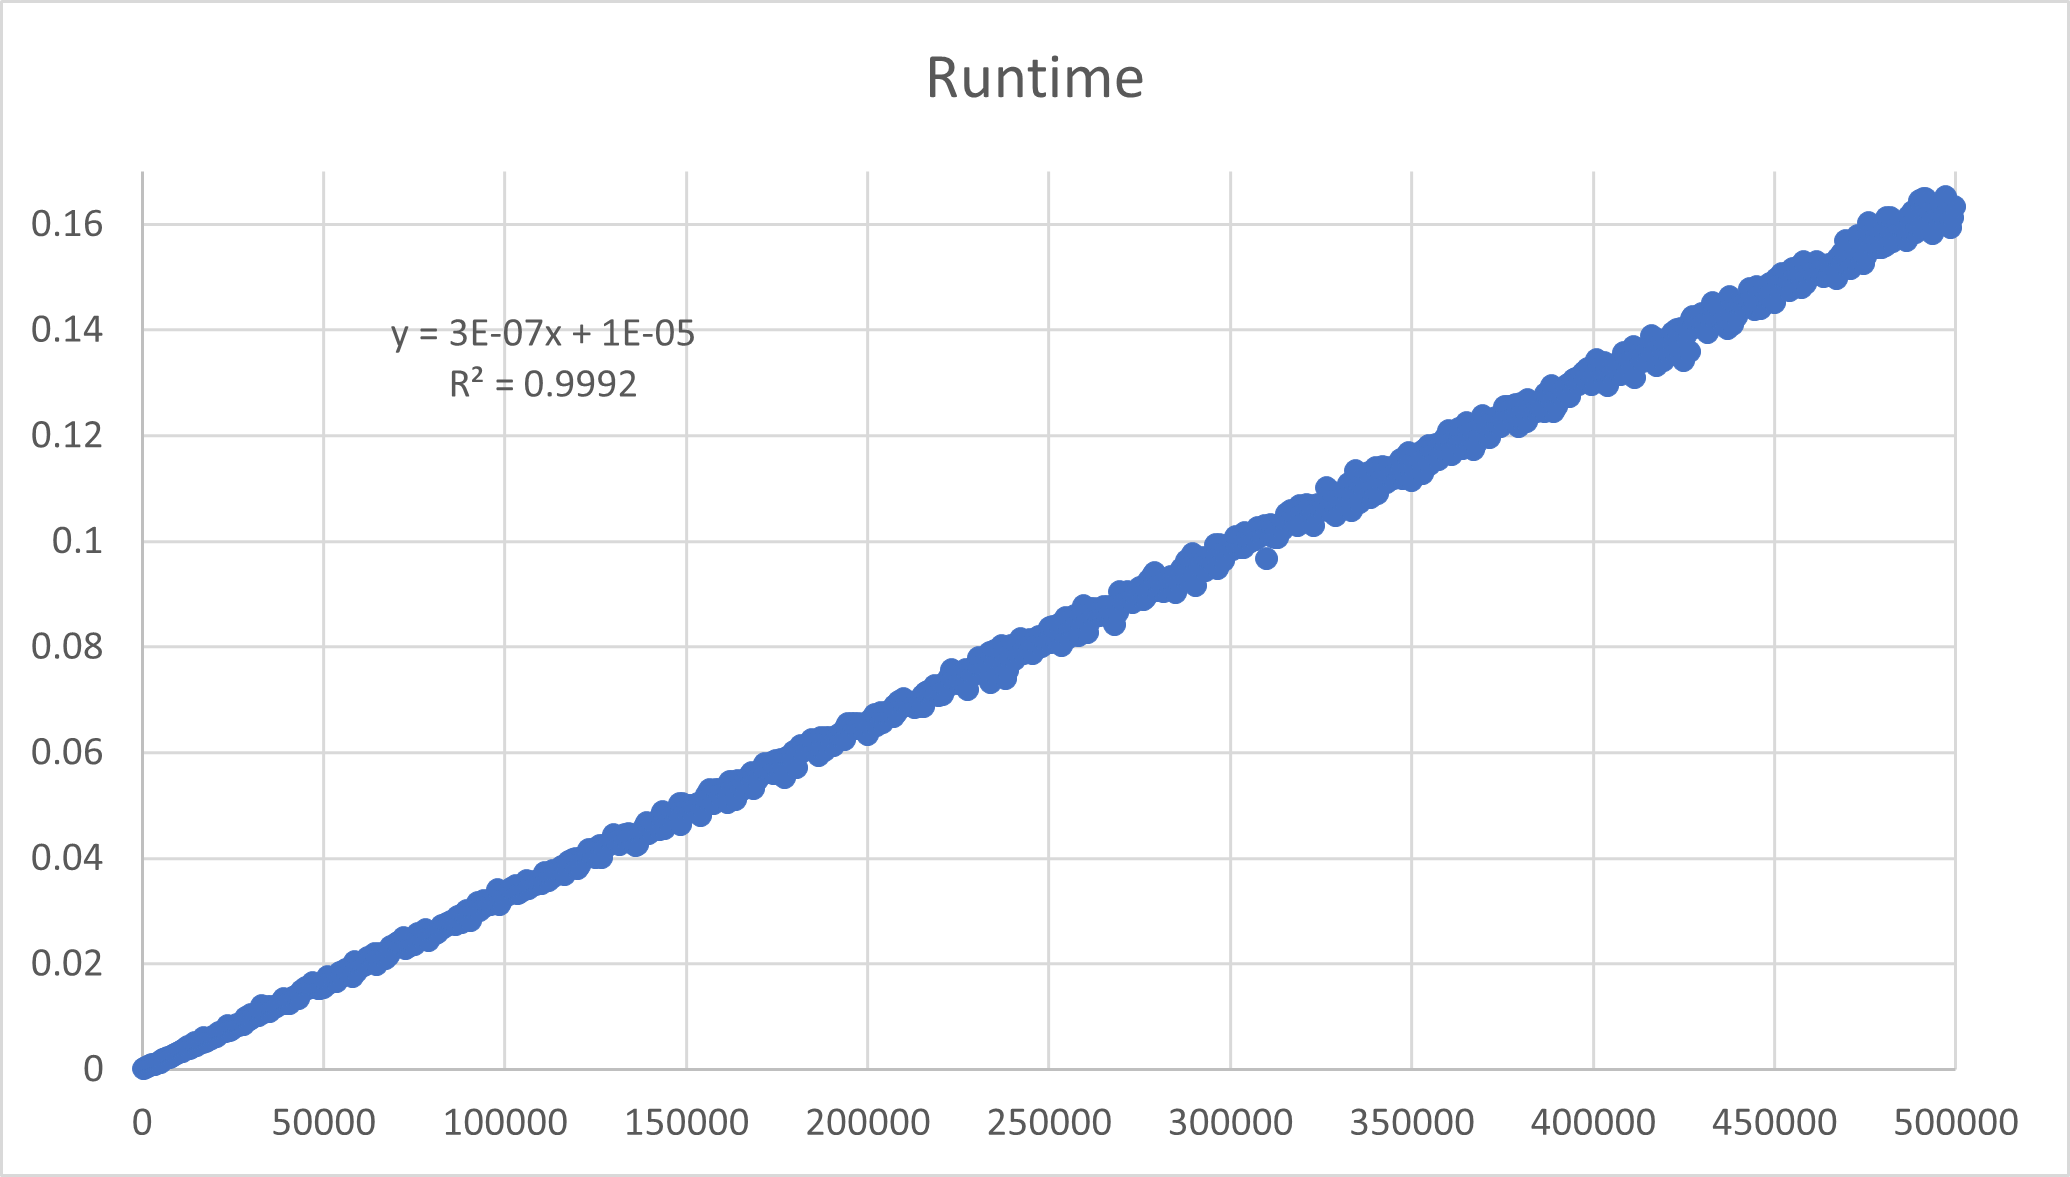
\includegraphics[width=0.6\textwidth,height=\textheight,keepaspectratio]{fn_Tn}
\caption{linear fitting for $f(n)$}
\label{Figure: fn_1}
\end{figure}
\noindent Therefore, we can conclude that $f(n) = O(n)$. 

\subsection{\(g(n)\)}
When we graph the data set for $g(n)$, the trend line appears to be polynomial. From the chart below we can see that the $R^2$ is 0.9883 for the quadratic equation. 

\begin{figure}[H]
\centering
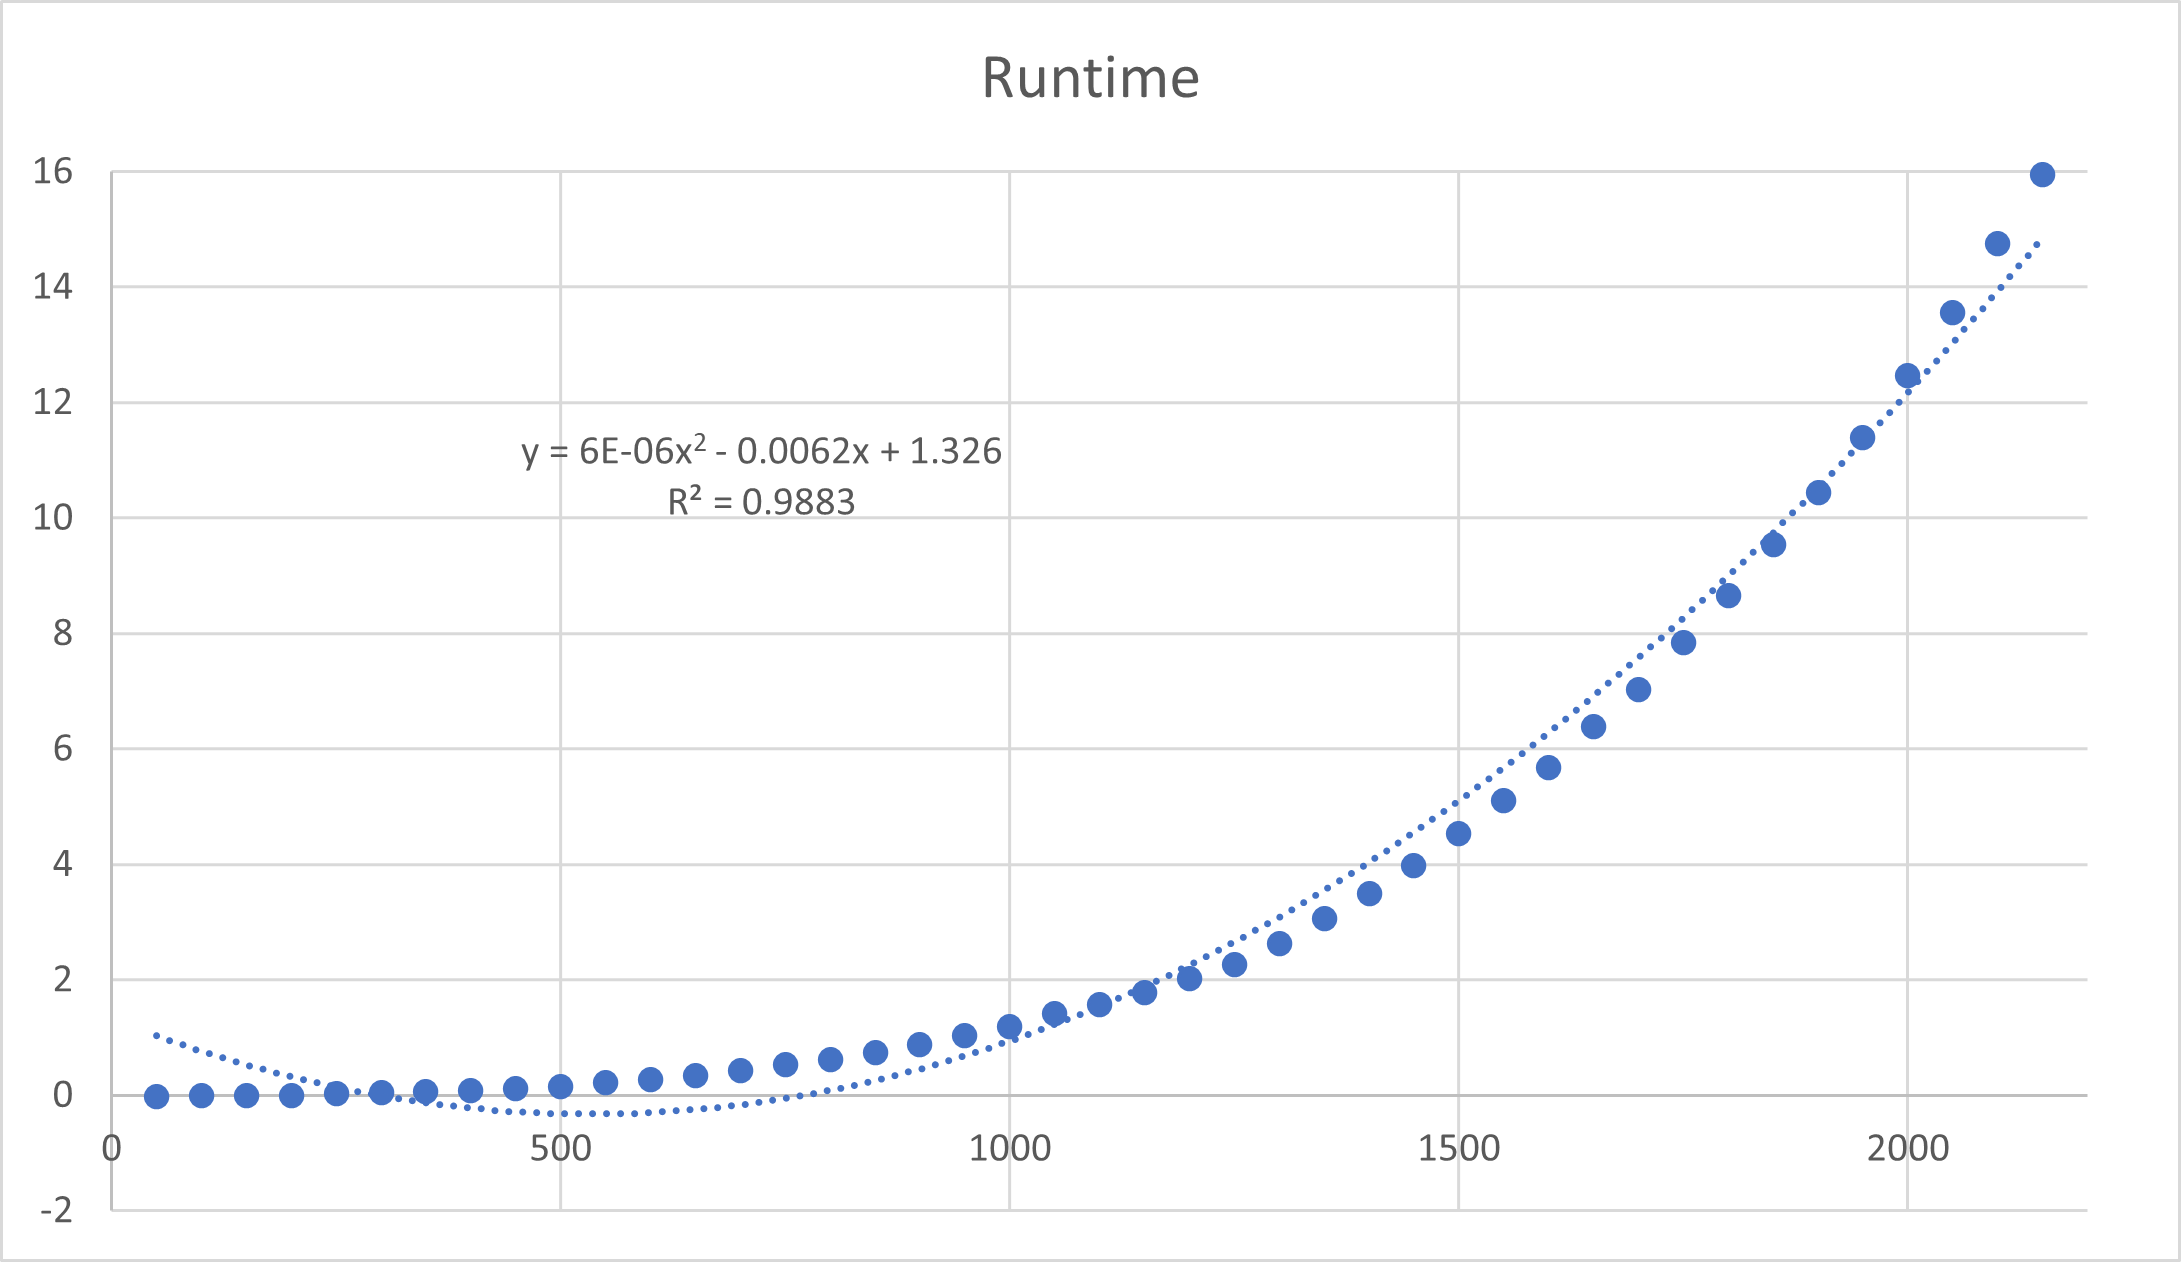
\includegraphics[width=0.6\textwidth,height=\textheight,keepaspectratio]{gn_Tn}
\caption{polynomial fitting for $g(n)$}
\label{Figure: gn_1}
\end{figure}

\noindent We will try to improve the $R^2$ by finding the value of $k$ in $T(n) = cn^k$. We do so by taking the logarithm of both sides of this equation: $\log{T}=\log{c}+k\log{n}$ and plotting $\log{T}$ against $\log{n}$. 

\begin{figure}[H]
\centering
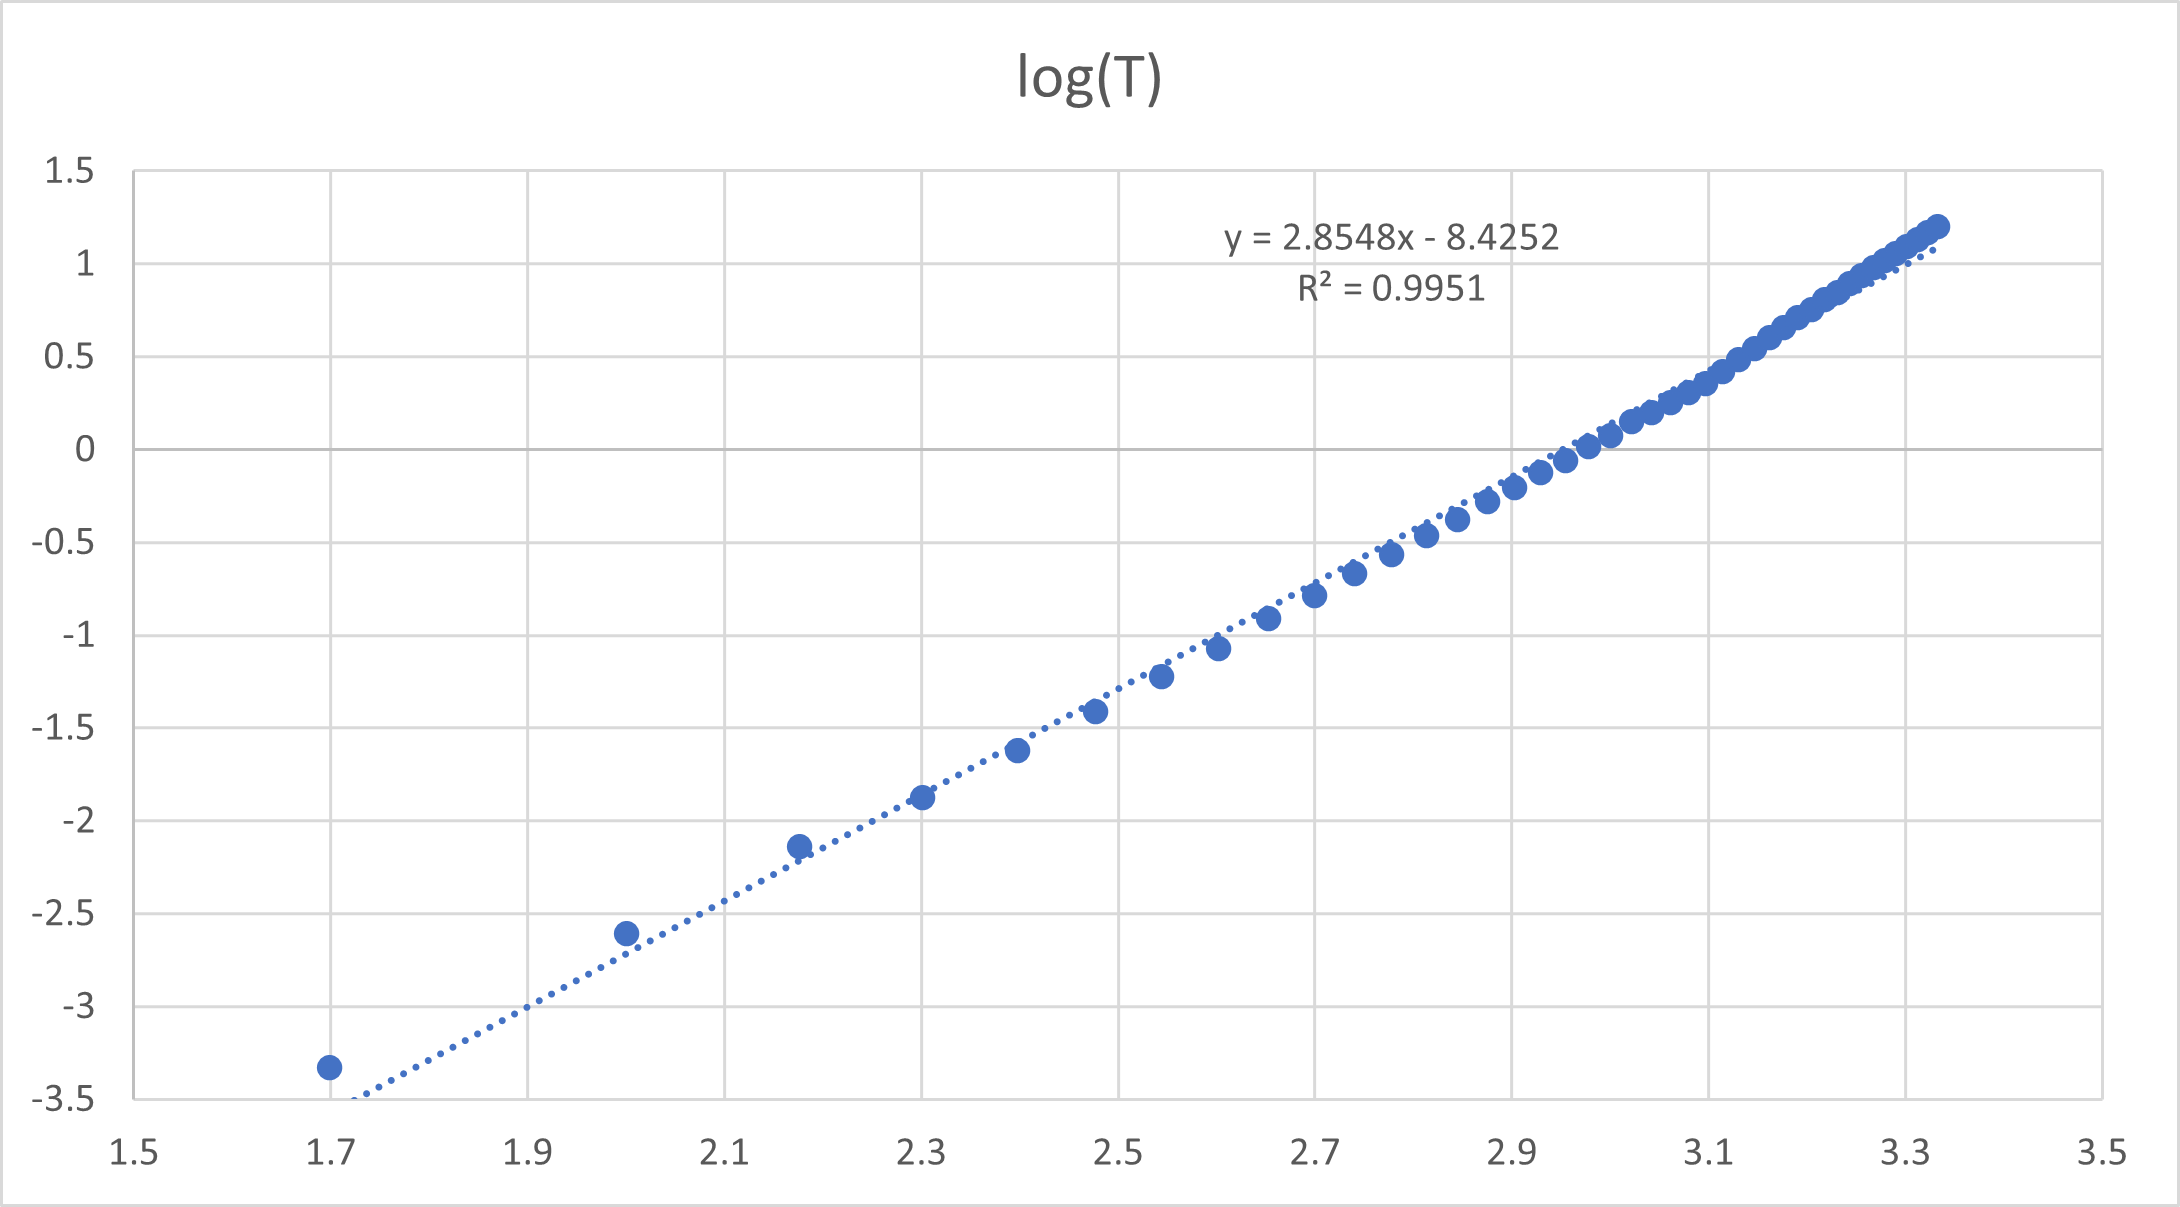
\includegraphics[width=0.6\textwidth,height=\textheight,keepaspectratio]{gn_logT}
\caption{polynomial fitting for $\log{T}$}
\label{Figure: gn_2}
\end{figure}

\noindent When we choose a linear trend line for this relation, we see that $k$, the slope, is 2.8548, which is closer to 3. When we recalculate the polynomial trend line for the original data with $k=3$, we see that this is a better fit.

\begin{figure}[H]
\centering
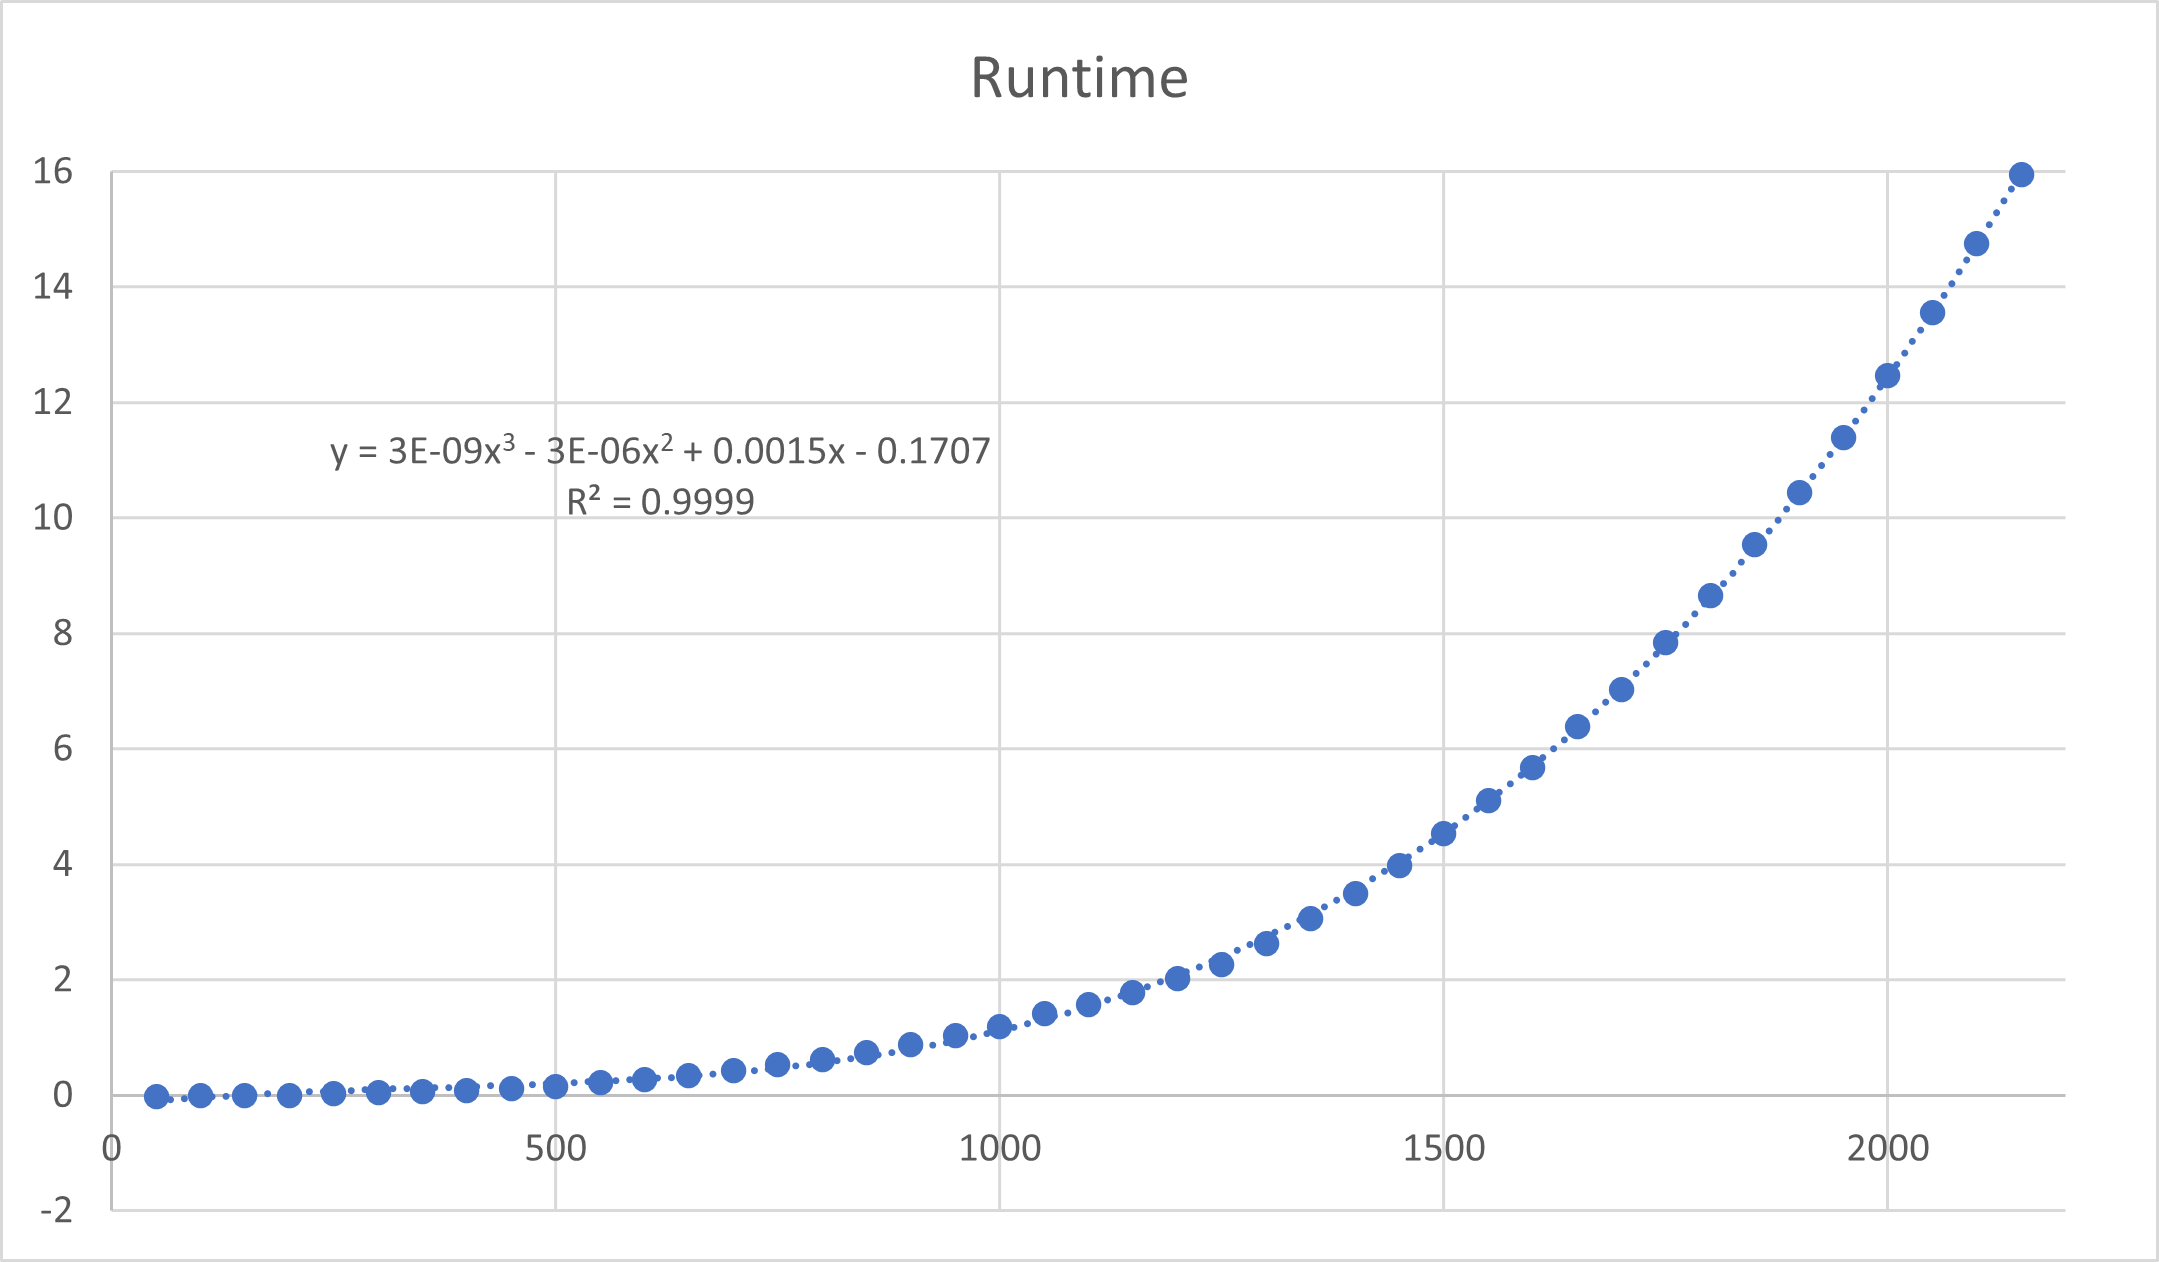
\includegraphics[width=0.6\textwidth,height=\textheight,keepaspectratio]{gn_Tn2}
\caption{linear fitting for $g(n)$}
\label{Figure: gn_3}
\end{figure}

\noindent Here, the $R^2$ is 0.9999, which is a very good result. Therefore we can conclude that $g(n) = O(n^3)$.

\subsection{\(h(n)\)}
When we graph the data set for $h(n)$, the trend line appears to be linear. From the chart below we can see that the $R^2$ is 0.9976 for the linear equation. This is already pretty good, but we might be able to improve it.

\begin{figure}[H]
\centering
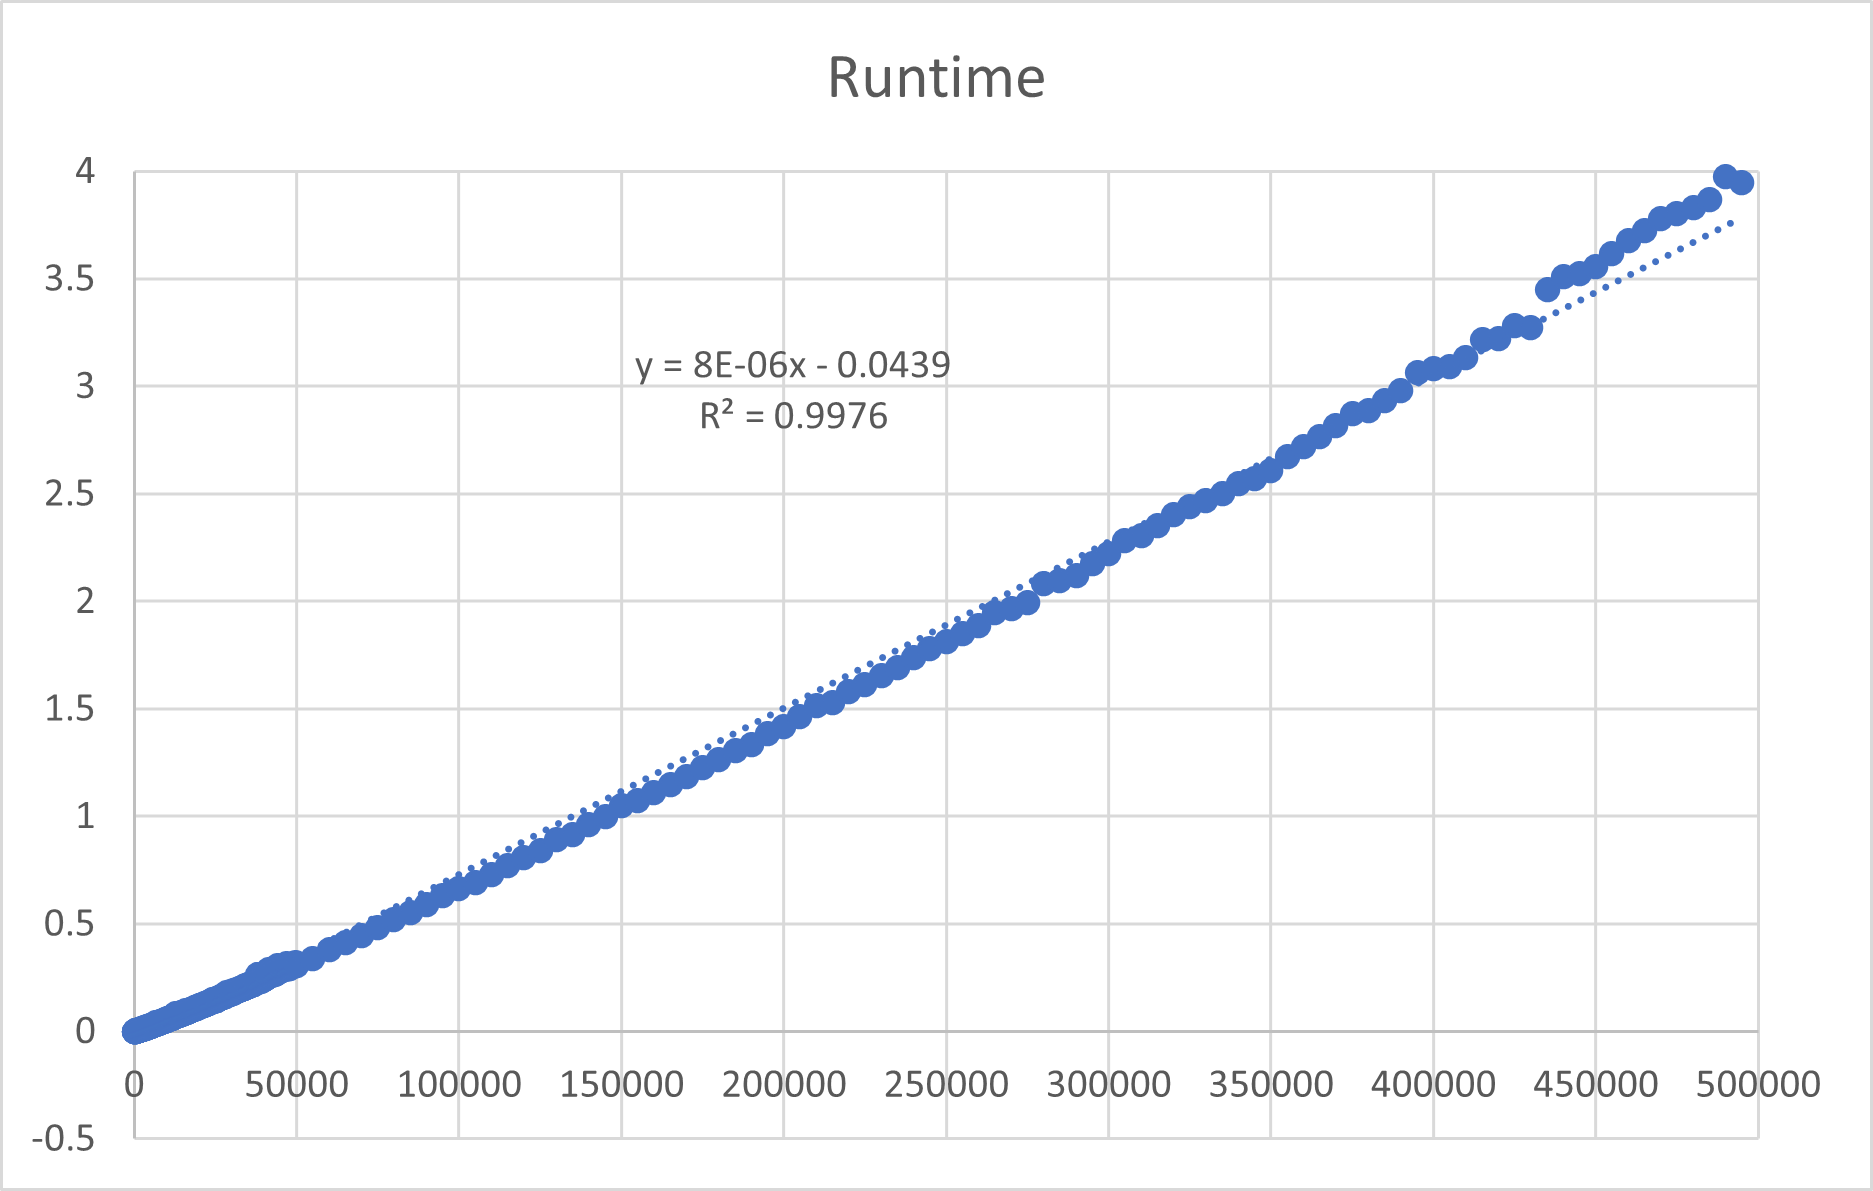
\includegraphics[width=0.6\textwidth,height=\textheight,keepaspectratio]{hn_Tn}
\caption{linear fitting for $h(n)$}
\label{Figure: hn_1}
\end{figure}

\noindent First, we will check the value of $k$ in $T(n) = cn^k$. We do so by taking the logarithm of both sides of this equation: $\log{T}=\log{c}+k\log{n}$ and plotting $\log{T}$ against $\log{n}$. 

\begin{figure}[H]
\centering
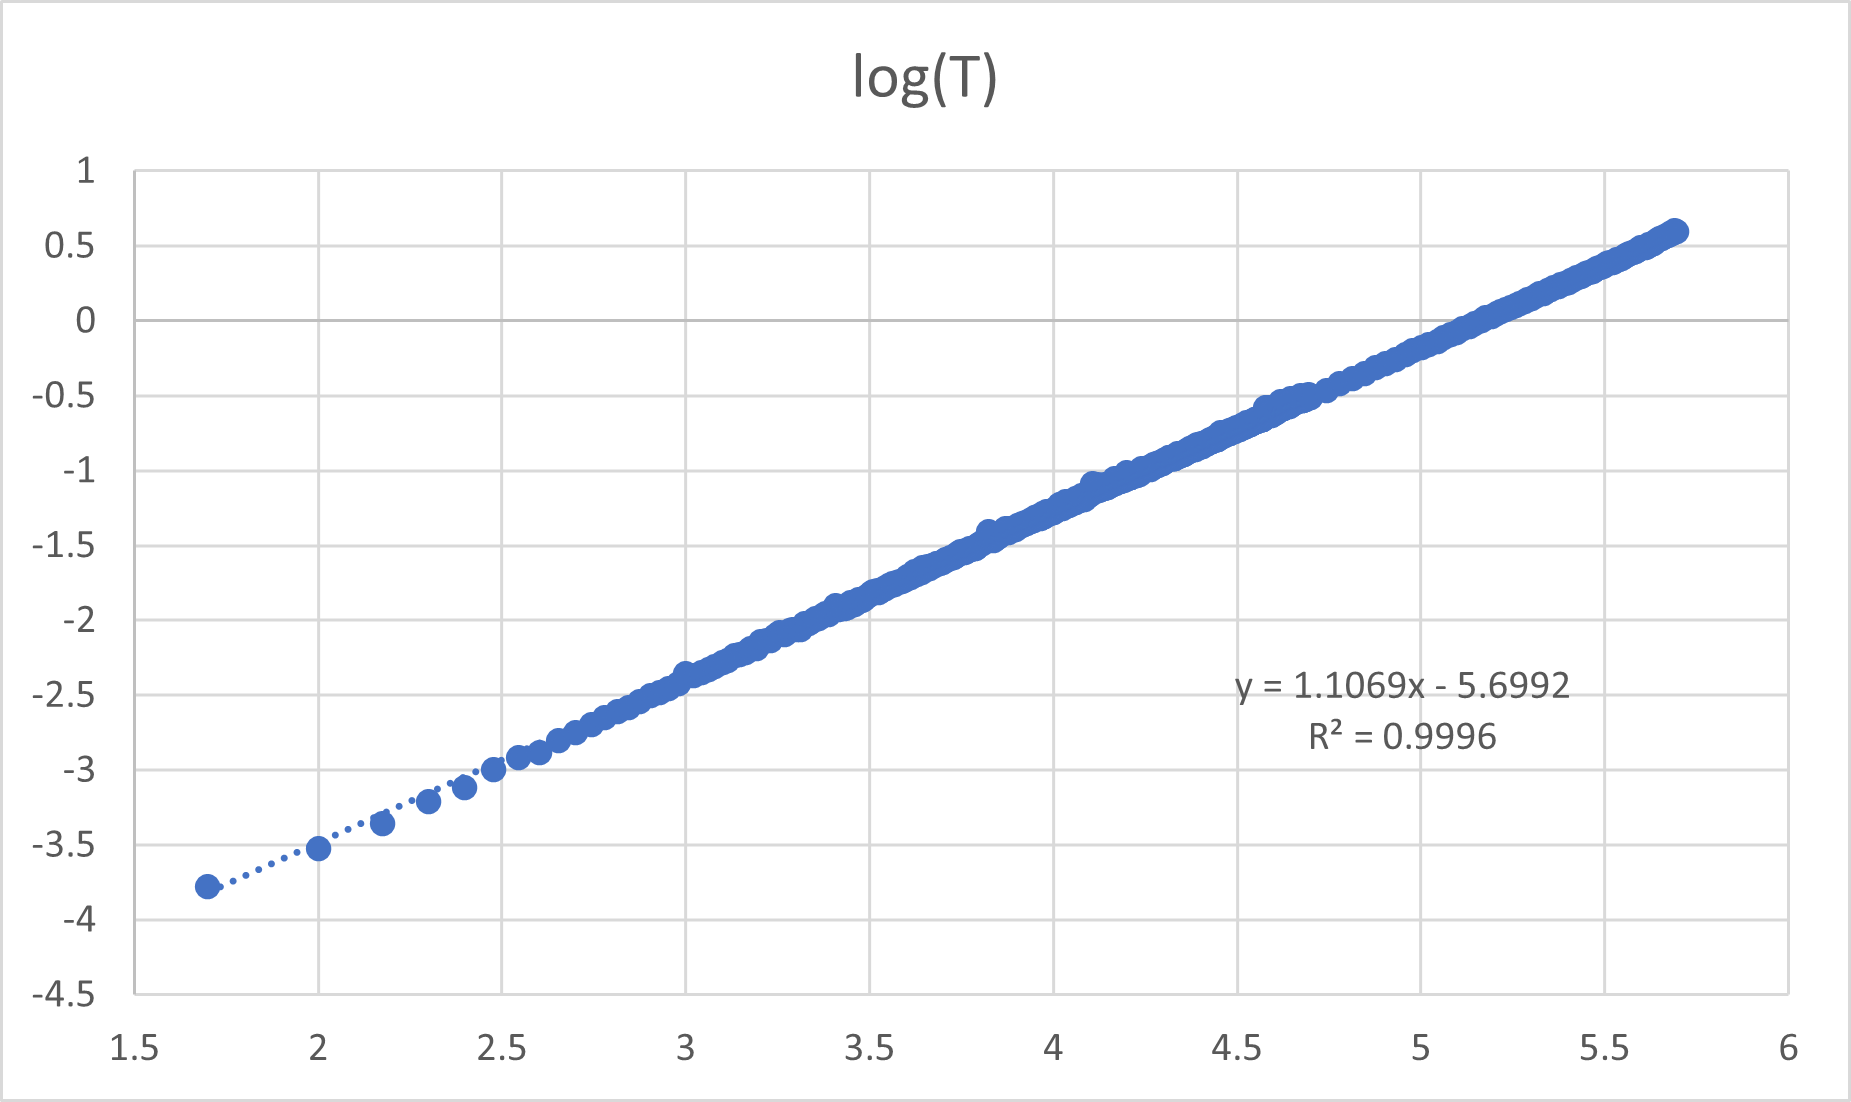
\includegraphics[width=0.6\textwidth,height=\textheight,keepaspectratio]{hn_logT}
\caption{linear fitting for $\log{T}$}
\label{Figure: hn_2}
\end{figure}

\noindent When we choose a linear trend line for this relation, we see that $k$, the slope, is 1.1069. Since $k$ represents the exponent on $n$ in the original data set, this makes the time complexity almost linear. However, $O(n\log{n})$ may be a better fit than $O(n)$. We can check which is better by plotting $\frac{T(n)}{n}$ against $n$. If $T(n) = cn$, then the resulting graph $\frac{T(n)}{n} = c$, will be linear. If $T(n) = cn\log{n}$, then the resulting graph $\frac{T(n)}{n} = c\log{n}$, will be logarithmic.

\begin{figure}[H]
\centering
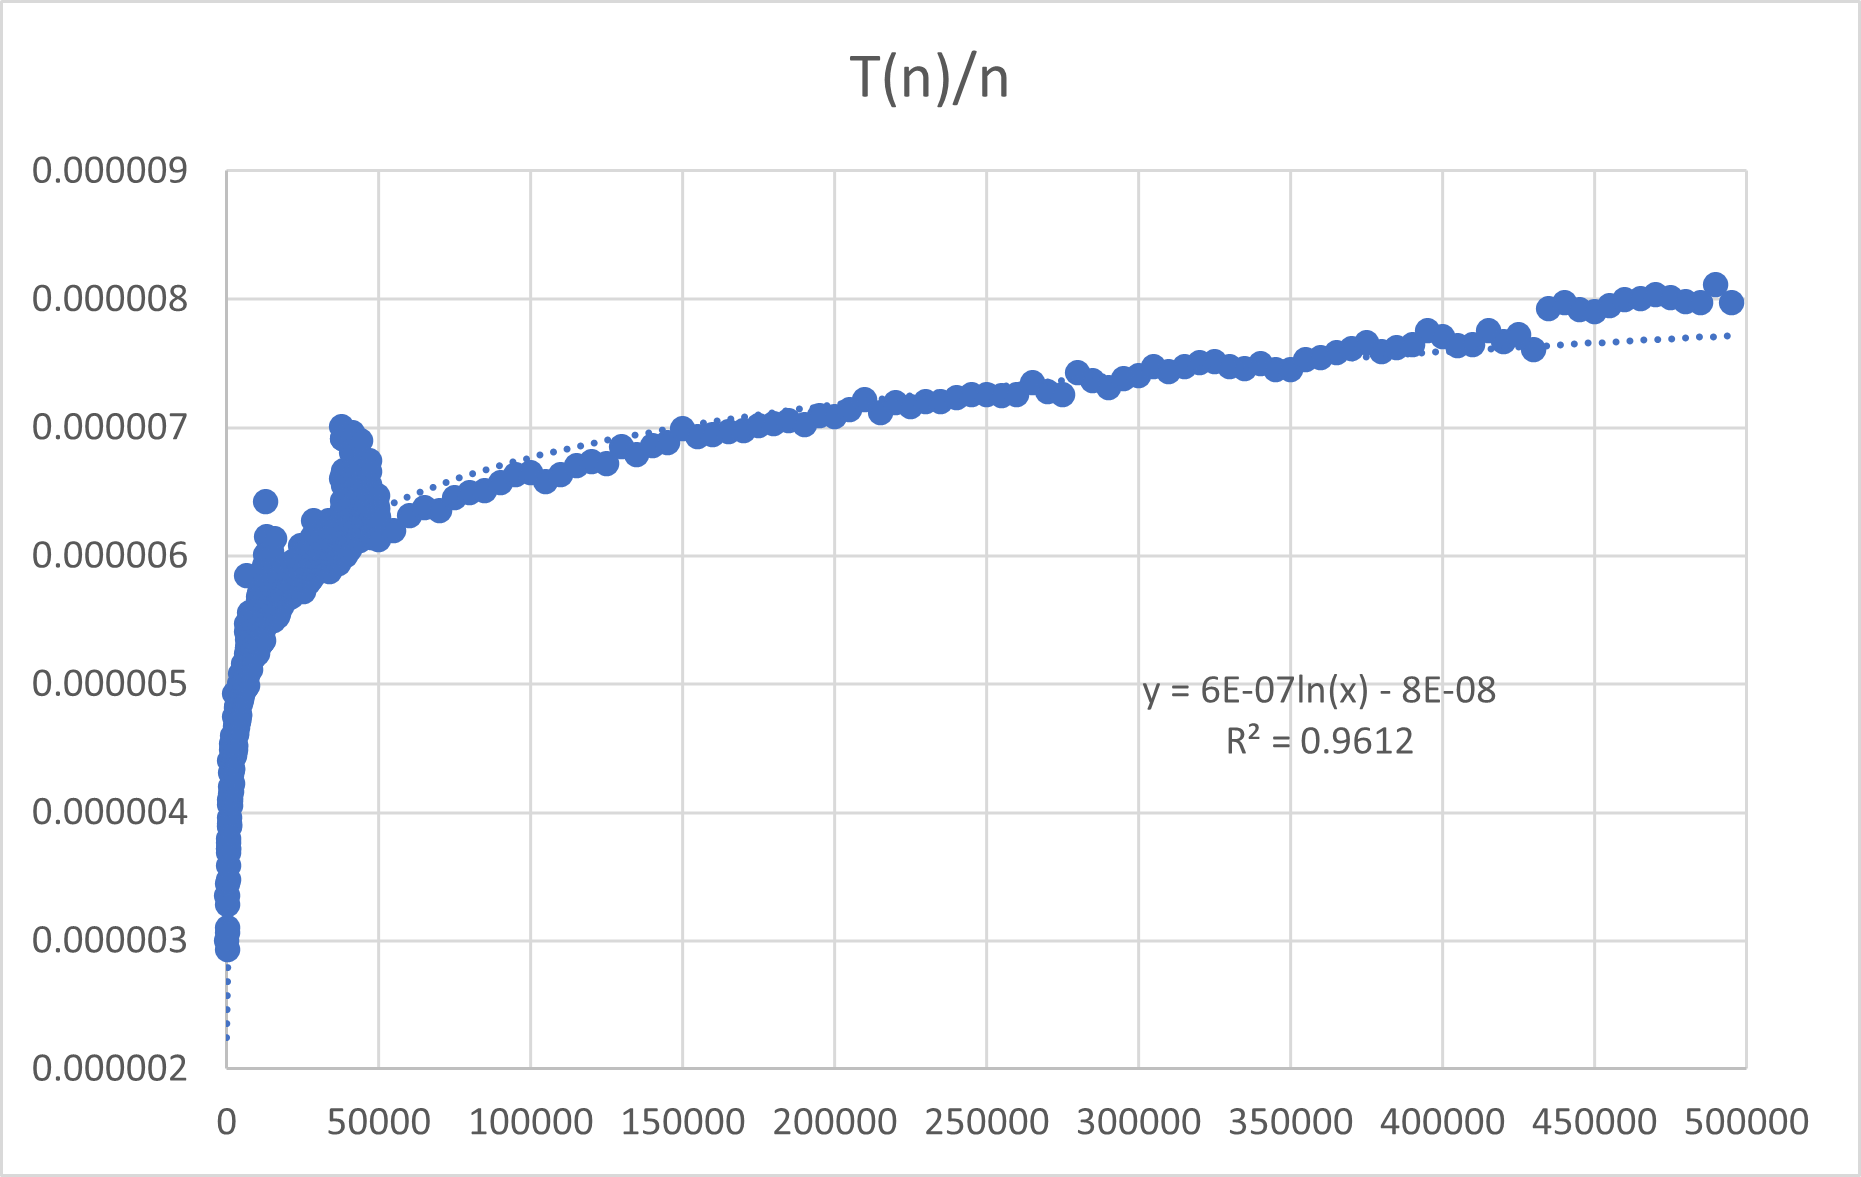
\includegraphics[width=0.6\textwidth,height=\textheight,keepaspectratio]{hn_Tn_n}
\caption{logarithmic fitting for $h(n)$}
\label{Figure: hn_3}
\end{figure}

\noindent The resulting graph appears to be logarithmic. The $R^2$ is 0.9612 for the logarithmic trend line. Therefore we can conclude that $h(n) = O(n\log{n})$.

\section{Python Lists}

To start, I would like to explain how each of the list methods is tested and evaluated. As specified in the .copy() instructions, the "timeit" library must be used. For the purpose of keeping the results consistent, I employed the library throughout the experiments. I used the function timeit.repeat() with parameters generating a total of 100 data points for a single input value. This data is then averaged and exported to a .csv file which is then analyzed in excel to determine the trend line and function complexity. The code to the "timer" is provided below and only changes slightly for each list method being analyzed.
\scriptsize
\begin{verbatim}
def timer(index):
  if __name__ == '__main__':
    import timeit
    print("timing for {} runs".format(index))
    return timeit.repeat("arrayGenApp({})".format(index), setup="from __main__ import arrayGenApp", repeat=10, number=5)
\end{verbatim}
\normalsize

\subsection{Copy}
For all three methods in question, very similar testing methods were selected. Since complexity is measured in the "big O" notation, where N is the number of inputs, the overall trend is seen by testing a relatively small number of inputs. 

I decided to start at an list size of 1 and multiply the subsequent list by 10 each time until the list is 1 million in size. Later, I  added additional data points starting at 3 and following similar steps to make my data more complete. 

\footnotesize
\begin{verbatim}
                                  timing for 1 runs
                                  timing for 3 runs
                                  timing for 10 runs
                                  timing for 30 runs
                                  timing for 100 runs
                                  ...
\end{verbatim}
\normalsize
  
The contents of the lists were different for each method tested. In the case of .copy() the list consisted of random integers between 0 and the size of the list being generated:

\footnotesize
\begin{verbatim}
import random

def arrayGenApp(upperLimit):
  j = 0
  arr = []

  while (j < upperLimit):
    arr.append(random.randint(0,upperLimit))
    j += 1

  return arr
\end{verbatim}
\normalsize

After generating the lists and measuring the time it took to .copy() each one of them, I received data which I plotted on the graph below. The data was plotted with a log scale to properly show the trend.

The initial flat section is consistent with the similar experiments found online and can be disregarded when analyzing the later data points. 

\begin{figure}[H]
\centering
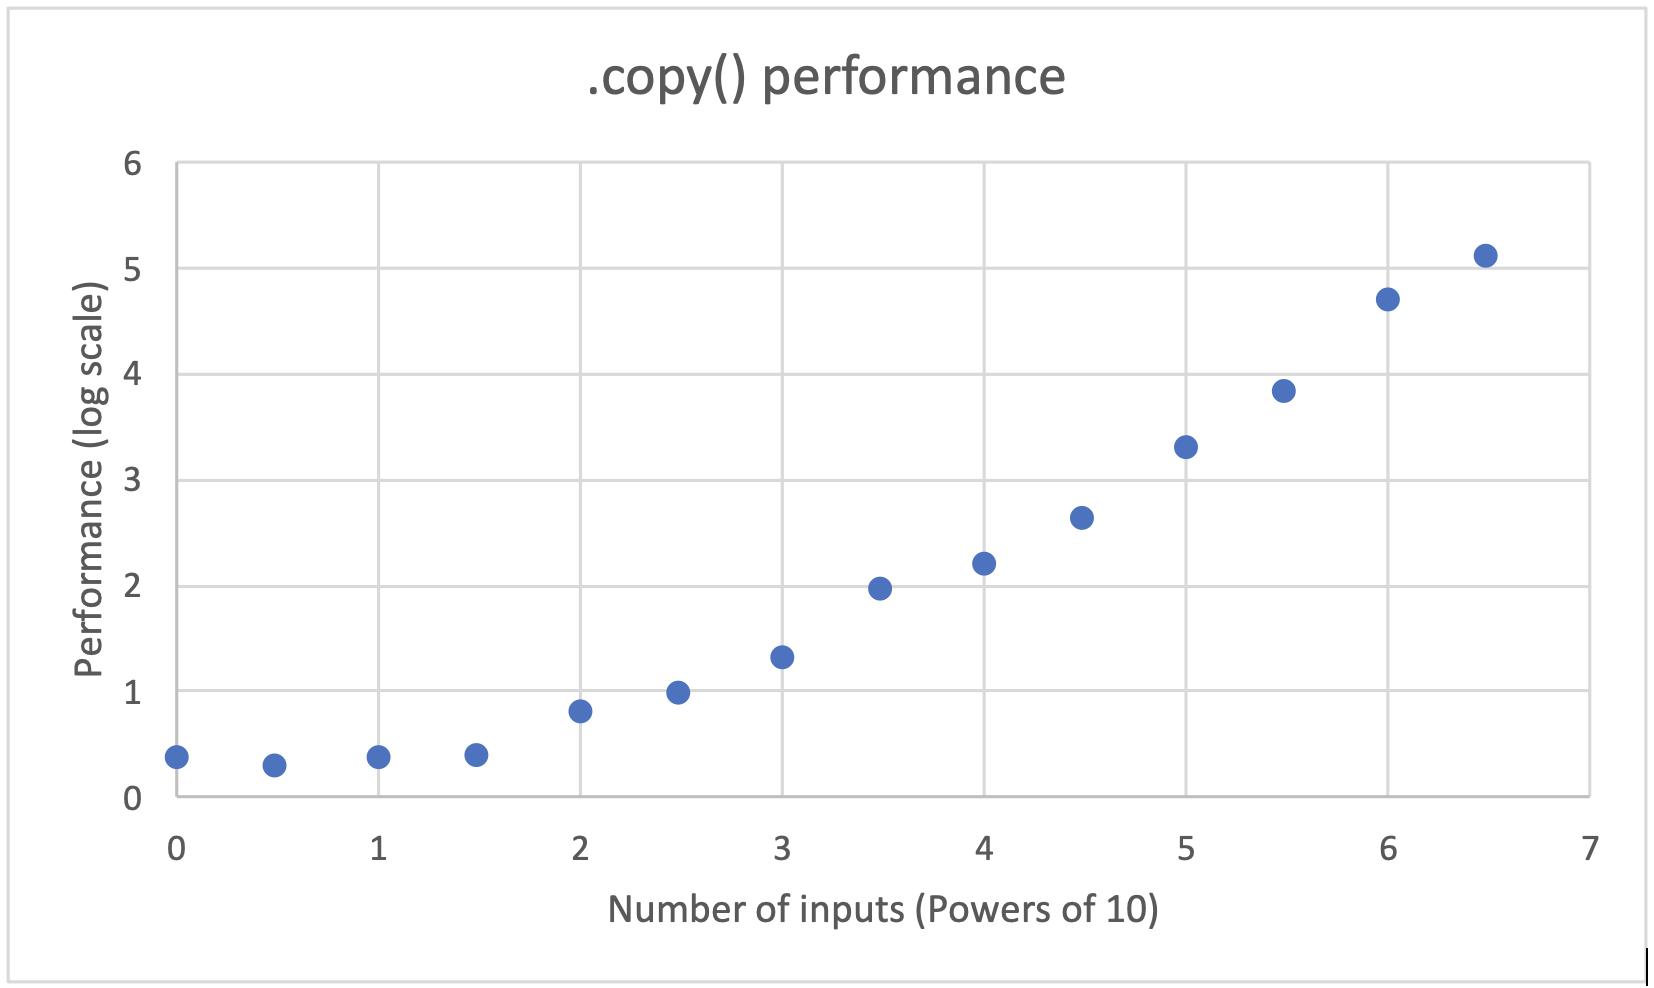
\includegraphics[width=0.6\textwidth,height=\textheight,keepaspectratio]{copygraph.png}
\caption{.copy() performance}
\label{Figure: copygraph}
\end{figure}

Based on official documentation, python's .copy() method runs in O(n) time [1] which is verified by the linear time complexity seen in the graph. This means that if we double an array size, it would take, on average, double the time to make a copy of it. 

\footnotesize
\begin{verbatim}
def copy(array):

  arrCpy = array.copy()

  return arrCpy
\end{verbatim}
\normalsize

Since array.copy() iterates over each object in an list, adding references to a new list, it is expected that the runtime would be linear.

\subsection{Lookups}

Lookups used a similar testing method to the one described in .copy(). This time, each list consisted of values from 0 to the upper limit in a natural order. For example, an list of size 10 had the values 0,1,2,...8,9. After consulting with the TA's, this was the method I decided to use as it provided a better estimate of lookups for python lists.

\footnotesize
\begin{verbatim}
def arrayGenApp(upperLimit): #values in array increasing
  j = 0
  arr = []
  
  while (j < upperLimit):
      arr.append(j)
      j += 1

  return arr
\end{verbatim}
\normalsize

My prediction for the runtime was that the method would not depend on the size of the list, meaning it would run in constant time O(1). For each lookup the algorithm does not need to traverse the list, instead, it would directly access the element with the given index. 

\footnotesize
\begin{verbatim}
def arrayLook(array):
  i = 0
  while (i < len(array)): 
    array[i]
    i += 1
\end{verbatim}
\normalsize

The first time we conducted this experiment, we realized that the method described in the question does not effectively test the lookup method. Using one million-length list does not test the lookup complexity for lists of varying sizes, only varying indices. Therefore we redesigned the experiment to 
measure the time it would take to look up each value in different size lists. 

Not only would this determine if the lookup method is dependent on list size, but also whether it is affected by the length of the variable being accessed. Since with my testing strategy, a larger list would have larger values stored within it.

\begin{figure}[H]
\centering
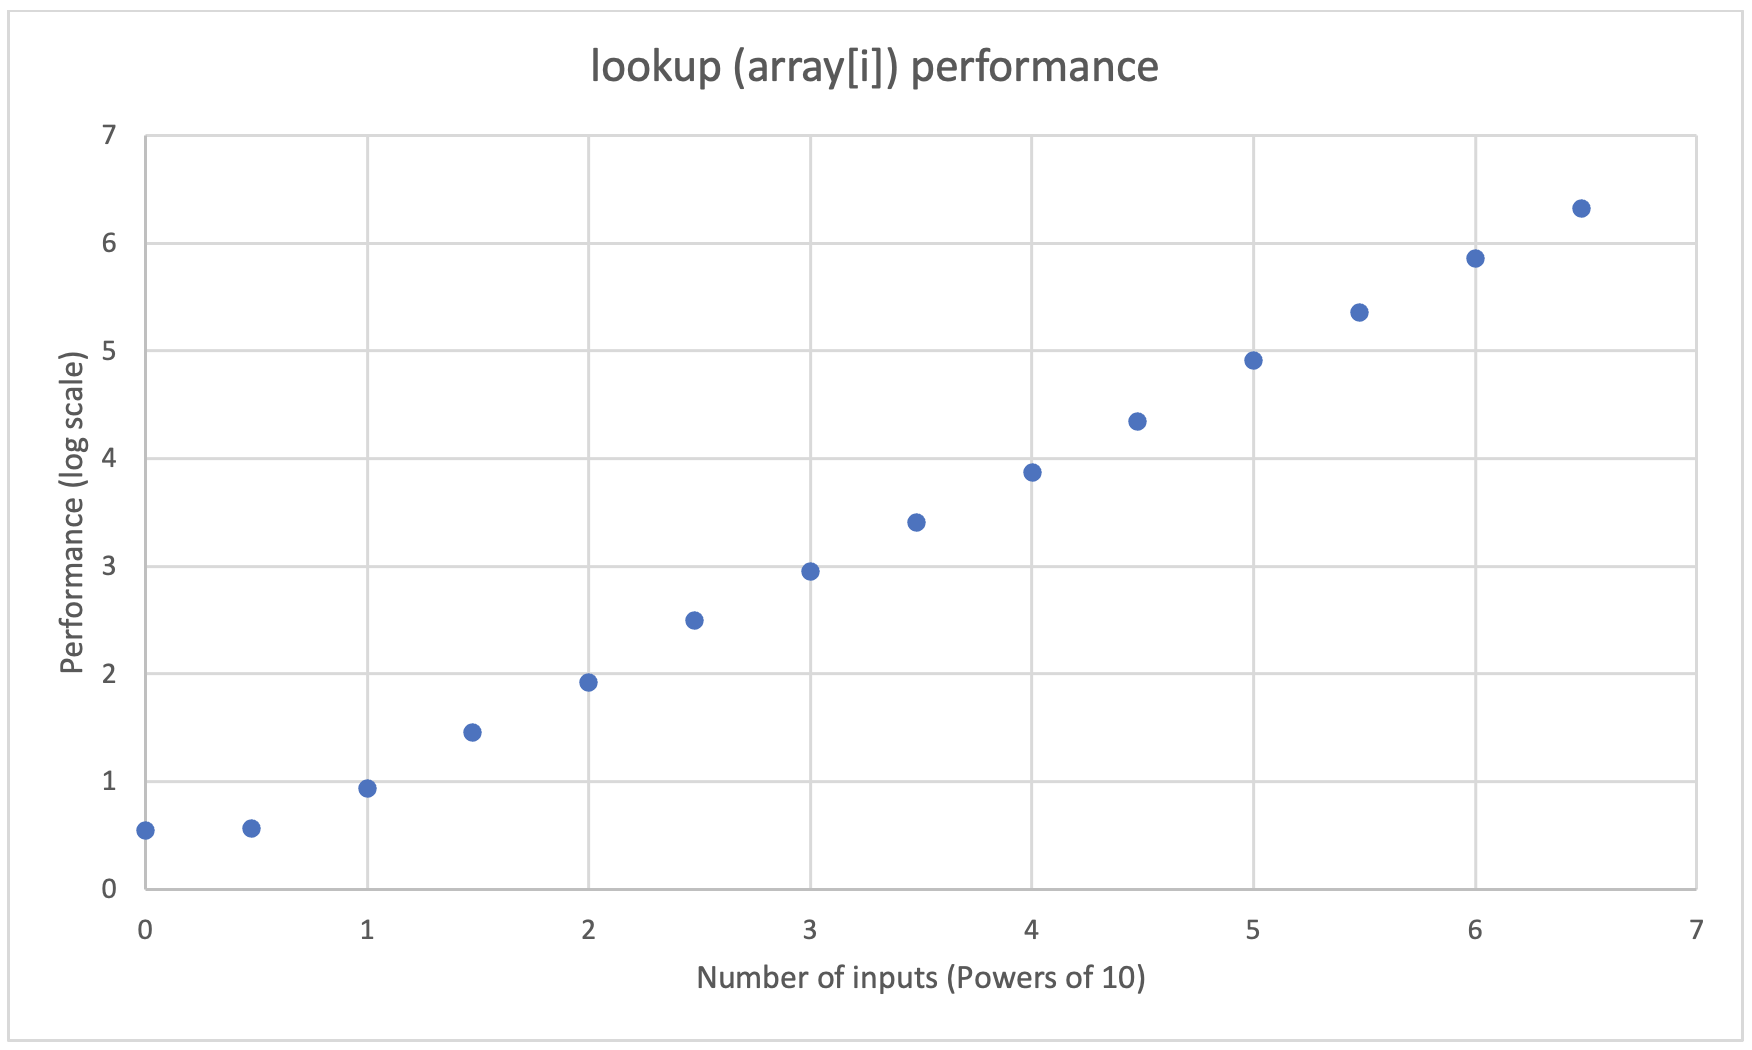
\includegraphics[width=0.6\textwidth,height=\textheight,keepaspectratio]{lookupgraph.png}
\caption{array[i] (lookup) performance}
\label{Figure: lookupgraph}
\end{figure}

As we can see from the above chart, the time taken to perform $n$ lookups increases linearly with respect to $n$. For each added lookup call, the time increases by a constant value. Therefore, our data suggests that lookup runs in $O(1)$. From the chart we can also see that the size of the element being accessed does not affect the performance of lookup. If the size of the element being accessed affected performance, we would see a quadratic relation instead of a linear one. This is because python lists are actually implemented as an array of pointers, which are all the same size [2].

\subsection{Append}

Similar to the lookup method, the procedure described in the lab document does not adequately control all possible variables and therefore would not produce an accurate result. By measuring the time it takes to append individual values, we will inevitably encounter flaws in the data due to the nature of lists in general. 

Since python lists are dynamic, meaning that their lengths are changeable, some append operations would take significantly more time than others. For example, if we started with a dynamic list of size 4, we could append 4 elements to it, and each operation would take constant time. Yet appending a fifth element onto that list would take longer as the list would have to create a new list of double the current size (8), copy the old elements onto the new list, and then add the new element. 

\footnotesize
\begin{verbatim}
def arrayGenApp(upperLimit): #values in array increasing
  j = 0
  arr = []
  
  while (j < upperLimit):
      arr.append(1)
      j += 1

  return arr
\end{verbatim}
\normalsize

Based on this evidence and a consultation with a TA I used the method I described when working on Lookups here. This method involves measuring the time it would take to create lists of different sizes using the .append() method and then plotting the data. The generated lists would progressively get bigger following the pattern seen in the .copy() method to ensure an accurate evaluation.

\footnotesize
\begin{verbatim}
i = 1
j = 3
  while (i < 1000001):
    logtocsv(i, average(timer(i)))
    logtocsv(j, average(timer(j)))
    
    i *= 10
    j *= 10
\end{verbatim}
\normalsize

The method employed here allows us to take care of the amortized analysis efficiently and elegantly, arriving at the correct conclusion. 

\begin{figure}[H]
\centering
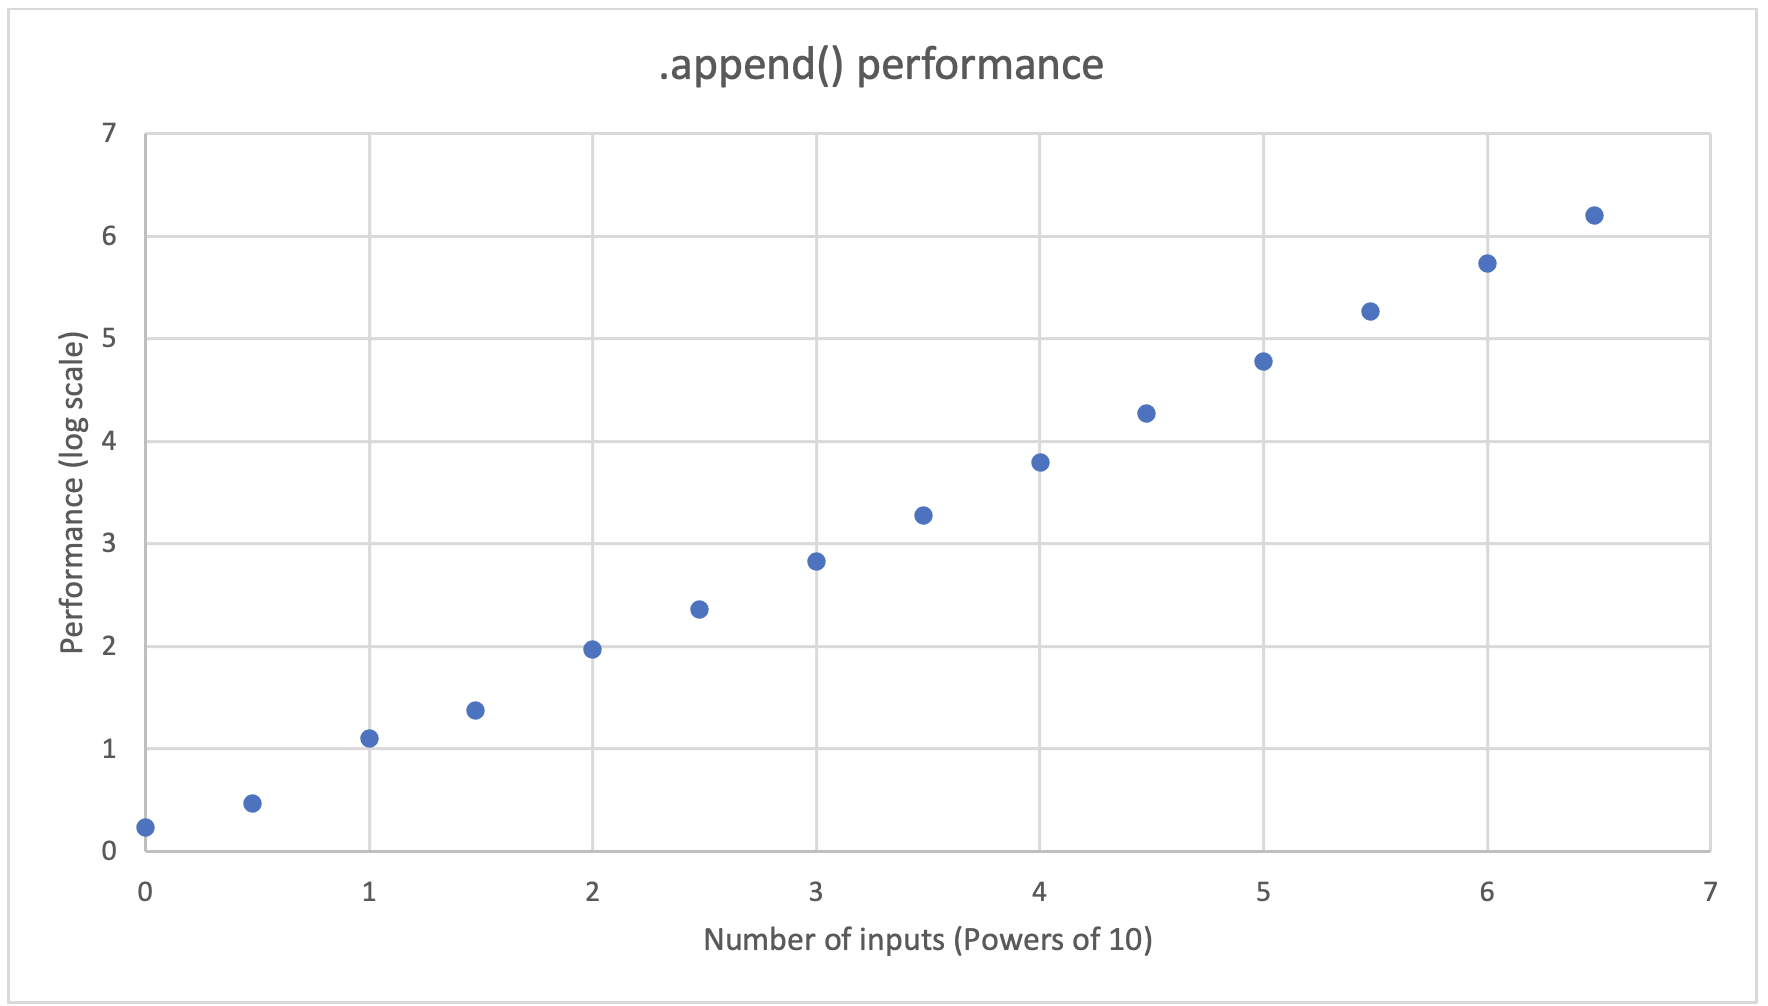
\includegraphics[width=0.6\textwidth,height=\textheight,keepaspectratio]{appendgraph.png}
\caption{.append() performance}
\label{Figure: appendgraph}
\end{figure}

Based on the data seen in the graph above we can conclude that the complexity is linear which is consistent with our hypothesis and official documentation [1].

\section{Conclusion}

For each method being tested, the analyzed data is consistent with the provided reference, as well as additional online sources. The complexity of O(n) for .append() and .copy() methods are demonstrated by the linear models graphed in the figures 8 and 10. The general case for the lookup method is similarly explained in figure 9 and its complexity is determined.

\newpage\section*{References}
\begin{enumerate}[label={[\arabic*]}]
\item	TimeComplexity. (2020, August 18). Python Wiki. Retrieved from \newline https://wiki.python.org/moin/TimeComplexity
\item	Design and History FAQ — Python 3.10.2 documentation. (n.d.). Python Docs. Retrieved from https://docs.python.org/3/faq/design.html
\end{enumerate}

\end{document}

